\subsection{Tuning experiments}

Figure~\ref{fig:bag-of-tasks-experiment} shows timing results for the
bag-of-tasks example.  Each plot considers a particular choice for the number
of intervals, |n|, and the number of tasks, |nTasks|.  The x-axis considers
different numbers of workers, and the y-axis gives the times taken.  Each run
used unbounded buffered channels.  Each observation performed $2^{27}/\sm{n}$
runs.

%%%%%

\begin{figure}
\begin{center}
\begin{tikzpicture}
\begin{semilogxaxis}[
%  title = Timing experiment on the numerical integration example,
  ylabel = Time (ms),
%  legend pos = north east,
  legend style={at={(0.70,0.98)}},
  height = 0.55\textheight,
  width = 0.85\textwidth,
  scaled ticks = false,
%  title = Experiment on the numerical integration bag-of-tasks example.,
  xlabel = Number of workers,
  log basis x=2,
  ymin = 500,
  ymax = 5000
]
\addplot+[error bars/.cd, y dir=both,y explicit] coordinates {
  (1,5450.6101748) +- (0,12.650706471088398)
  (2,3056.442098428571) +- (0,28.737642840384968)
  (4,2154.3953815666664) +- (0,20.693639090142195)
  (8,3350.65515325) +- (0,32.63665761213119)
  (16,5594.300504181818) +- (0,50.32486183690076)
  (32,7475.9241562) +- (0,48.417094704814176)
  (64,9986.346586285716) +- (0,98.09082844202608)
};
\addlegendentry{$\sm n = 2^{18}$, $\sm{nTasks} = 2^{9}$}
\addplot+[error bars/.cd, y dir=both,y explicit] coordinates {
  (1,5007.675461) +- (0,13.686326182482928)
  (2,2731.0204338333333) +- (0,23.35039731606894)
  (4,1616.8292285185184) +- (0,16.138829689738955)
  (8,1865.081054625) +- (0,18.53227480228986)
  (16,2701.604537571429) +- (0,25.969680061097936)
  (32,3680.565586090909) +- (0,36.210743908097214)
  (64,4568.203701666667) +- (0,41.715695160489254)
};
\addlegendentry{$\sm n = 2^{20}$; $\sm{nTasks} = 2^{10}$}
\addplot+[error bars/.cd, y dir=both,y explicit] coordinates {
  (1,4884.6682636000005) +- (0,17.782427429822622)
  (2,2570.123440777778) +- (0,24.80872494458182)
  (4,1514.0846481400001) +- (0,31.850239055539483)
  (8,1263.6072703599998) +- (0,29.581306649002393)
  (16,1628.5271092424243) +- (0,15.899583168616081)
  (32,2100.7852361428572) +- (0,20.340306504248268)
  (64,2461.952226961538) +- (0,23.696128463145246)
};
\addlegendentry{$\sm n = 2^{22}$; $\sm{nTasks} = 2^{11}$}
\addplot+[error bars/.cd, y dir=both,y explicit] coordinates {
  (1,4922.292719333333) +- (0,38.37834775822396)
  (2,2677.5306812) +- (0,24.85402705231822)
  (4,1538.3950354400001) +- (0,17.909341023643474)
  (8,1070.5430969400002) +- (0,34.3563713210201)
  (16,1133.5246862000001) +- (0,9.883390535725946)
  (32,1373.7130467380953) +- (0,13.717792332933353)
  (64,1626.3286156818183) +- (0,16.00981709292464)
};
\addlegendentry{$\sm n = 2^{24}$; $\sm{nTasks} = 2^{12}$}
\addplot+[error bars/.cd, y dir=both,y explicit] coordinates {
  (1,5069.178585542857) +- (0,50.37213086034046)
  (2,2691.89330344) +- (0,37.767455164393304)
  (4,1530.5242046600001) +- (0,28.817161707223033)
  (8,1010.6285473400001) +- (0,32.66829660709502)
  (16,1017.41061254) +- (0,30.678738953720778)
  (32,1084.9625646) +- (0,15.169669087395743)
  (64,1244.38884936) +- (0,12.978136074354166)
};
\addlegendentry{$\sm n = 2^{26}$; $\sm{nTasks} = 2^{13}$}
\end{semilogxaxis}
\end{tikzpicture}

\end{center}
\caption{Experiments on the bag-of-tasks example.}
\label{fig:bag-of-tasks-experiment}
\end{figure}

%%%%%

It is useful to consider the quantity $\sm n / \sm{nTasks}$ for each plot,
i.e.~the number of intervals per tasks, which runs from $2^9$ to $2^{13}$ by
factors of~$2$.  This is a good measure of the computational cost of each
task.   For smaller values of this measure, the program achieves poor scaling,
being slower for eight workers than for four.  This is consistent with what we
saw earlier: the low computational cost of each task means that the channels
become congested.  However, for higher values of this measure, the program
scales better.  

%%%%%

Figure~\ref{fig:bag-of-tasks-experiment-2} gives results for experiments
considering the number of tasks to give each worker.  Each run used eight
workers, and unbounded buffered channels.  Each plot considers a particular
value for the number of intervals,~|n|.  The x-axis gives the average number
of tasks per worker.  Each observation is based on $2^{28}/\sm{n}$ runs.

\begin{figure}
% scala  tacp.trapezium.TrapeziumExperiment --doBagNumTasks --strict
\begin{center}
\begin{tikzpicture}
\begin{semilogxaxis}[
%  title = Timing experiment on the numerical integration example,
  ylabel = Time (ms),
%  legend pos = north east,
  legend style={at={(0.55,0.98)}},
  height = 0.55\textheight,
  width = 0.85\textwidth,
  scaled ticks = false,
%  title = Experiment on the numerical integration bag-of-tasks example considering the number of tasks.,
  xlabel = Tasks per worker,
  log basis x=2,
  ymax = 3800
]
\addplot+[error bars/.cd, y dir=both,y explicit] coordinates {
  (1,3352.5584418666667) +- (0,32.39018336931468)
  (2,3177.6074104) +- (0,30.03046065403267)
  (4,2825.346039153846) +- (0,26.578742030652567)
  (8,2633.3589845416664) +- (0,26.058560420431323)
  (16,2556.6023542105263) +- (0,25.525369128045856)
  (32,2602.1325810999997) +- (0,25.620813091083203)
  (64,2754.1994305999997) +- (0,26.43581717528377)
  (128,3386.6708786) +- (0,26.598870170170244)
  (256,4947.1010282) +- (0,48.25750793782477)
};
\addlegendentry{$\sm n = 2^{20}$}
\addplot+[error bars/.cd, y dir=both,y explicit] coordinates {
  (1,2430.0985353076926) +- (0,24.161751494140365)
  (2,2590.3529583000004) +- (0,25.299756842425655)
  (4,2153.021478857143) +- (0,21.273131359790593)
  (8,1925.8373171666667) +- (0,17.959884614345665)
  (16,1836.6189299722223) +- (0,18.19037513122588)
  (32,1825.1809766071428) +- (0,18.10857316008791)
  (64,1839.26816146875) +- (0,18.20233464725214)
  (128,1880.6876090666667) +- (0,18.619059018086812)
  (256,2134.17022104) +- (0,28.68720991042429)
};
\addlegendentry{$\sm n = 2^{22}$}
\addplot+[error bars/.cd, y dir=both,y explicit] coordinates {
  (1,2049.76257738) +- (0,20.246850253890152)
  (2,2428.827615181818) +- (0,24.25034273533704)
  (4,1977.1314379230769) +- (0,19.558354330713257)
  (8,1686.9642632222224) +- (0,16.774562309432827)
  (16,1573.5973083611111) +- (0,15.678148981214)
  (32,1562.8593507857145) +- (0,15.444602885745132)
  (64,1570.87964412) +- (0,18.331970500511368)
  (128,1558.21264084) +- (0,22.30355302530338)
  (256,1691.5533438599998) +- (0,32.58672115299523)
};
\addlegendentry{$\sm n = 2^{24}$}
%% \addplot+[error bars/.cd, y dir=both,y explicit] coordinates {
%%   (1,1925.447759847826) +- (0,19.18777386975458)
%%   (2,2400.668871714286) +- (0,23.39996657676753)
%%   (4,1921.7963885384615) +- (0,19.058506647775467)
%%   (8,1652.4909764285715) +- (0,16.169790819327602)
%%   (16,1502.772550652174) +- (0,14.76747235535448)
%%   (32,1524.1503742999998) +- (0,14.118010595497367)
%%   (64,1522.0211753636363) +- (0,15.055364262187124)
%%   (128,1464.9243361666668) +- (0,14.226315577346861)
%%   (256,1581.72356702) +- (0,26.315896274033975)
%% };
%% \addlegendentry{$\sm n = 2^{26}$}
\addplot+[error bars/.cd, y dir=both,y explicit] coordinates {
  (1,1853.7602047799999) +- (0,23.20821176816953)
  (2,2337.0621846153845) +- (0,21.871343828100212)
  (4,1899.366764) +- (0,18.96852892309966)
  (8,1634.8610090999998) +- (0,24.11141714793872)
  (16,1501.6389951400001) +- (0,19.394279658177584)
  (32,1491.06709548) +- (0,17.686753672081153)
  (64,1490.079240175) +- (0,14.677187086601563)
  (128,1494.2455339795918) +- (0,14.746633258811613)
  (256,1525.11317254) +- (0,27.009019402748162)
};
\addlegendentry{$\sm n = 2^{28}$}
\end{semilogxaxis}
\end{tikzpicture}

\end{center}
\caption{Experiments on the bag-of-tasks example, considering the number of
  tasks per worker.}
\label{fig:bag-of-tasks-experiment-2}
\end{figure}

Each plot shows a decrease in time as the number of tasks per worker increases
from two to about sixteen.  Having more tasks allows for better load
balancing.  However, beyond a certain point, increasing the number of tasks
makes the program slower: at this point, the channel communication is becoming
a bottleneck again.

Most of the plots show that using an average of two tasks per worker is slower
than just one, which may seem surprising.  I investigated this by arranging
for each worker to print the number of tasks it processed.  When the average
is one task per worker, it is nearly always the case that each worker indeed
executes exactly one task; the difference in times taken by workers is not
very large in this case.  However, when the average is two tasks per worker,
it is normally the case that at least one (slow) worker performs only one
task, and so another worker performs three; the latter worker therefore takes
considerably longer than the others, and this increases the overall running
time.

It is worth noting that each of the plots has a fairly wide U-shape.  For the
lower three plots, there is little difference between $2^4$ and $2^7$ tasks
per worker.  This is a good situation, as it suggests the program is fairly
stable with respect to changes in speed of workers, for example caused by
different hardware. 

Experiments on the 32-core server gave similar results, except in order to
benefit from the additional machine threads, each task needs to be larger.

% \framebox{casteret}

